\section{Experimental Results}

\begin{figure}
\centering
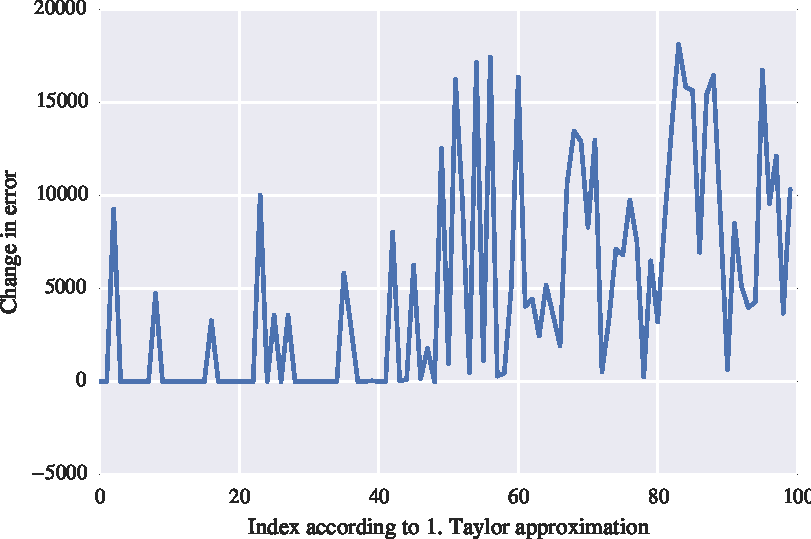
\includegraphics[width=0.6\linewidth]{error1.pdf}
\caption{Error when using first order Taylor Series approximation.}
\label{fig:error1}
\end{figure}

\begin{figure}
\centering
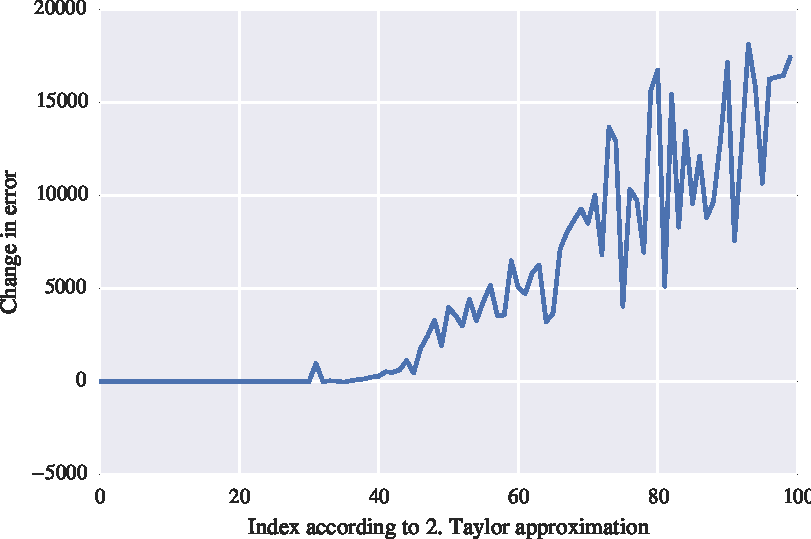
\includegraphics[width=0.6\linewidth]{error2.pdf}
\caption{Error when using second order Taylor Series approximation.}
\label{fig:error2}
\end{figure}

\begin{figure}
\centering
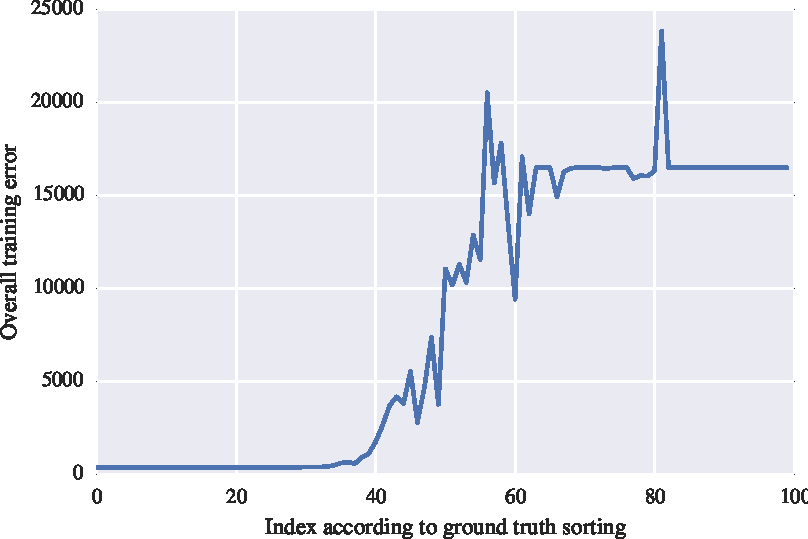
\includegraphics[width=0.6\linewidth]{improvement1.pdf}
\caption{Improvement of the training error when using the brute force ordering.}
\label{fig:improvement1}
\end{figure}

\begin{figure}
\centering
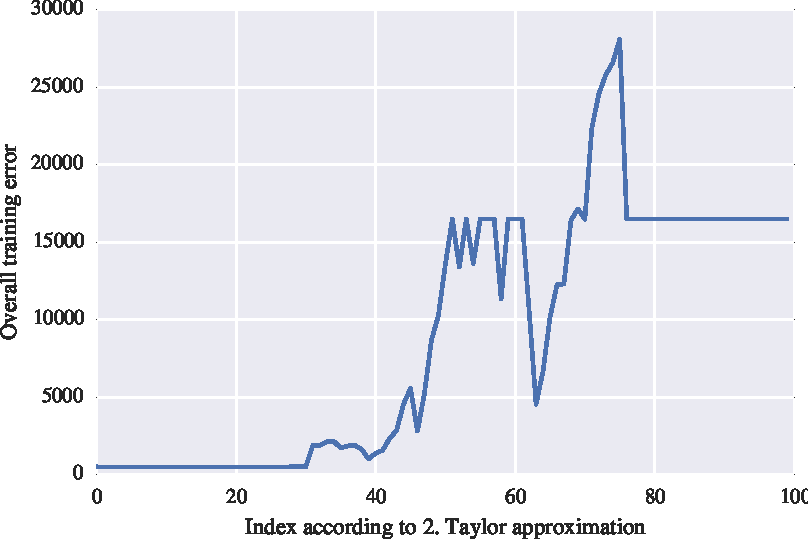
\includegraphics[width=0.6\linewidth]{improvement3.pdf}
\caption{Improvement of the training error when using the second order Taylor approximation.}
\label{fig:improvement3}
\end{figure}
